%%TODO: IF THIS GETS IN, CITE MY THESIS (since I present an early version
%of this idea in my background and copied some text from there)

% Template for ICIP-2018 paper; to be used with:
%          spconf.sty  - ICASSP/ICIP LaTeX style file, and
%          IEEEbib.bst - IEEE bibliography style file.
% --------------------------------------------------------------------------
\documentclass{article}
\usepackage{spconf,amsmath,amssymb,amsfonts,amsthm,graphicx}
\usepackage{algorithm}% http://ctan.org/pkg/algorithms
\usepackage{algpseudocode}% http://ctan.org/pkg/algorithmicx


\graphicspath{{Figures/}}
\newcommand{\argmin}{\operatornamewithlimits{argmin}}
\newcommand{\argmax}{\operatornamewithlimits{argmax}}


\title{Eulerian Synthesis of Slow Motion Periodic Videos}

%
% Single address.
% ---------------
\name{Author(s) Name(s)\thanks{Thanks to XYZ agency for funding.}}
\address{Author Affiliation(s)}
%
% For example:
% ------------
%\address{School\\
%	Department\\
%	Address}
%
% Two addresses (uncomment and modify for two-address case).
% ----------------------------------------------------------
%\twoauthors
%  {A. Author-one, B. Author-two\sthanks{Thanks to XYZ agency for funding.}}
%	{School A-B\\
%	Department A-B\\
%	Address A-B}
%  {C. Author-three, D. Author-four\sthanks{The fourth author performed the work
%	while at ...}}
%	{School C-D\\
%	Department C-D\\
%	Address C-D}
%
\begin{document}
%\ninept
%
\maketitle
%


\begin{abstract}
Abstract
\end{abstract}
%
\begin{keywords}
One, two, three, four, five
\end{keywords}
%


\section{Introduction}

\begin{figure}[h!]
\centering
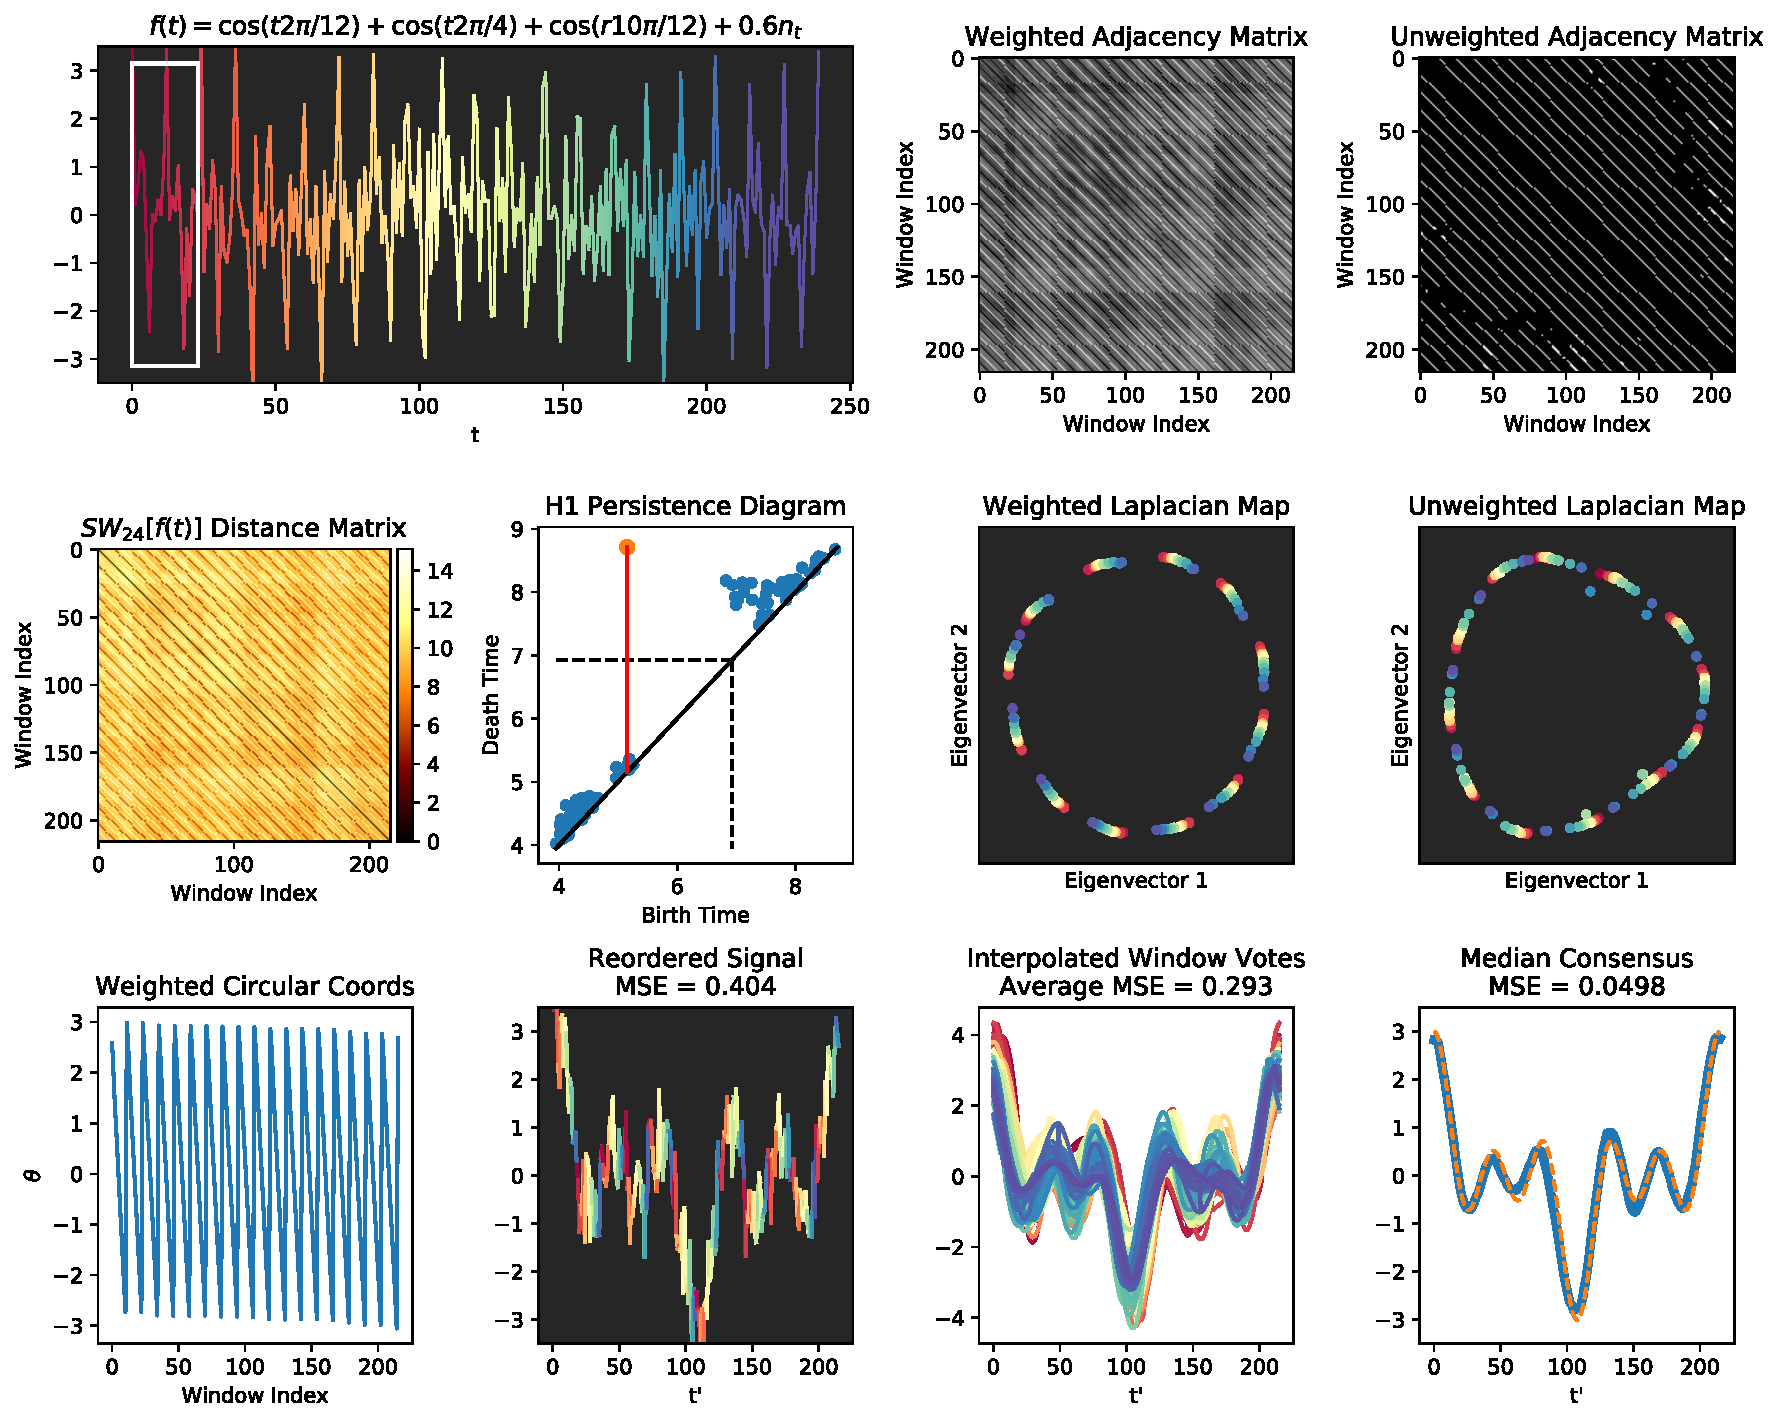
\includegraphics[width=\columnwidth]{1DExample.pdf}
\caption{An illustration of our technique on a 1D periodic time series with additive Gaussian noise ($n_t \in \mathcal{N}(0, 1)$).  We estimate the period to be 24 (a multiple of the fundamental frequency), and perform a 24-length sliding window embedding.  From this, we use the mean of the birth and death time of the largest persistence dot (row 2, column 2) to autotune the spatial bandwidth for the graph Laplacian (upper right two figures for the weighted and unweighted Laplacian), from which we derive a map to the circle (middle, right two plots).  From this, we derive circular coordinates, which we can use to do a simple reordering (row 3 column 2) or median consensus (row 3, column 3), using interpolated votes from all windows interleaved by the coordinates (row 3, column 2). }
\label{fig:ConceptFigure}
\end{figure}

Repetitive, periodic motions are ubiquitous in our world, such as animal locomotion (walking/flapping/slithering/swimming), mechanical motions (wheels spinning, pistons oscillating), biological rhythms (heartbeat, breathing), musical rhythms (drumming, feet tapping), etc.  In this work, we consider videos of periodic motion.  One avenue of interest is to analyze these videos in fine detail, such as for characterizing subtle progressions of blood flow in the face during a heartbeat for medical diagnostic purposes.  It may also be important to understand and visualize variations from cycle to cycle, such as in a repetitive automated action on an assembly line, where too much variation could indicate the onset of failure, or in athletic activities for optimizing performance.  

Our approach is {\em Eulerian}; that is, we process the video pixel by pixel with no tracking.  Unlike Fourier-based Eulerian motion video processing tools (\cite{wu2012eulerian, wadhwa2013phase}), however, we take a {\em geometric} approach by quantifying {\em sliding window embeddings} of our videos (Section~\ref{sec:slidingwindow}).  Sliding window embeddings of periodic time series form samples of a topological loop \cite{perea2015sliding}, as do generalized multivariate sliding windows on periodic video data \cite{traliehigh, tralie2017quasi}.  This implies that, at the right scale, a nearest neighbor graph built on the sliding window point cloud should be approximately a circle graph, even if the overall extrinsic geometry is quite complicated.  Bearing this in mind, we use Laplacian eigenmaps \cite{belkin2003laplacian} of this embedding to construct maps from these point clouds to the circle, or {\em circular coordinates} (Section~\ref{sec:laplacian}).  In particular, each sliding window is assigned a phase $\phi \in [0, 2\pi]$.  To autotune the scale at which Laplacian eigenmaps are built, we use topological data analysis \cite{edelsbrunner2000topological,edelsbrunner2008persistent,edelsbrunner2010computational,carlsson2009topology,ghrist2014elementary} to automatically find the scale at which the most prominent loop in the data occurs.

Once we have extracted a phase for each window, we use this information to reorder the content of the video.  We also exploit the sliding window structure to have different windows vote on the final pixels in each frame of the template (Section~\ref{sec:cyclereordering}).  As an illustration, Figure~\ref{fig:ConceptFigure} shows an example of our technique on a sampled periodic time series (i.e. single pixel grayscale video).  There are only 12 samples per period in the original signal, so the details of each period coarse and noisy.  However, once they are re-sorted, we get a nice, fine-detailed representation of one period.  The extension of this technique to videos will be described in detail in Section~\ref{sec:methods}.


\section{Releated Work}
Our technique unifies many disparate ideas that have appeared before in different contexts, in addition to the references we mentioned in the introduction.  Sliding window embeddings, or ``delay reconstructions,'' have found a diverse array of applications in activity recognition \cite{frank2010activity,venkataraman2016shape}, gene expression data \cite{perea2015sw1pers}, EEG analysis \cite{stam2005nonlinear, plesnik2014detection}, audio and music analysis \cite{herzel1994analysis,serra2009cross,bello2011measuring,traliemoebius}, video analysis \cite{schodl2000video, tralie2017quasi}, and motion capture analysis \cite{venkataraman2016shape}.  All of these works focus on analysis rather than synthesis, as we do, but there has been work using sliding window embeddings to synthesize ``video textures,'' or videos that repeat dynamics indefinitely \cite{schodl2000video}, which are similar in spirit to our infinitely looping periodic representatives.  The graph Laplacian, on the other hand, has been used to re-arrange images around a loop as a pre-processing step for structure from motion \cite{averbuch2015ringit}, and vector diffusion maps have been used to re-order the frames of microscope images a developing embryo around a loop \cite{dsilva2015diffusionvecordering}.  A different topological approach with cohomology circular coordinates\cite{de2011persistent} was used to parameterize a sliding window embedding of the Lorenz attractor \cite{de2012topological} and periodic activites in motion capture data \cite{vejdemo2015cohomological}.  Neural networks have also been trained to find circular coordinates \cite{levy2015live,anafi2017cyclops}.  Finally, perhaps the most related to our goal is work synthesizing seamless video loops by clustering pixels into different periods and adjusting them to loop through a common period \cite{Liao2013VideoLoops,Liao2015VideoLoops}.  TODO: talk about applications of TDA?



\section{Methods}
\label{sec:methods}

\begin{algorithm}[t]
  \caption{Sliding Window Video Loops}\label{alg:videoreordering}
  \begin{algorithmic}[1]
    \Procedure{ReorderVideo}{$X$, $L$, weighted, median} \\
    \Comment{$X$ is a $W \times H$ video $X$ with $N$ frames, an $N \times 3WH$ matrix}
    \State ($\theta, d) \gets$ CIRCCOORDS($X, L$)
    \State Perform SVD $X = USV^T$, $\hat{X} \gets US \in \mathbb{R}^{N \times N}$
    \State $\hat{Y} \gets SW_d[\hat{X}[n]] \in \mathbb{R}^{M \times N \times d}$, $M = N-d+1$
    \If {median}
        \State Order $\hat{Y}$ by $\theta$, line up each window in time, and linearly interpolate coordinates of $\hat{Y}$
        \State Do median consensus on aligned pixels of $\hat{Y}V^T$ \label{algline:medianconsensus}
    \Else
        \State Order first frames in each window by $\theta$
    \EndIf
    \EndProcedure
  \end{algorithmic}
\end{algorithm}


\begin{algorithm}[t]
    \caption{Laplacian Circular Coordinates}
    \begin{algorithmic}[1]
    \Procedure{CircCoords}{$X$, $L$}
    \State $\hat{X} \gets $ image pyramid level $L$ of $X$
    \State Perform SVD $\hat{X} = USV^T$, $Y \gets US \in \mathbb{R}^{N \times N}$
    \State $y \gets$ 1D ISOMAP($Y$) \cite{tenenbaum2000global}
    \State $d \gets$ fundamental period estimate of $y$ \cite{Mcleod05asmarter}
    \State $Z \gets SW_{d}[Y[n]] \in \mathbb{R}^{M \times N \times d}$, $M = N-d+1$

    \State $I \gets dgm_1[Z] = ((b_1, d_1), ... (b_k, d_k))$
    \State $i \gets \argmax_{i}[d_i - b_i]$, $\sigma \gets b_i + \frac{1}{2}(d_i - b_i)$
    \State $d_{ij} \gets ||Z_i - Z_j||_2$
    \If {weighted}
        \State $A_{ij} \gets e^{-d_{ij}^2/\sigma}$
    \Else
        \State $A_{ij} \gets \left\{ \begin{array}{cc} 1 & d_{ij} \leq \sigma \\ 0 & \text{otherwise} \end{array} \right\}$
    \EndIf
    \State $A_{ii} \gets 0, D_{ii} \gets \sum_{j=1}^M A_{ij}, D_{i, j \neq i} \gets 0$, $L \gets D - A$
    \State $v_1, v_2 \gets $ adjacent eigenvectors of $L$ with fewest zcs
    \State $\theta \gets \cos^{-1}(v_2/v_1)$\\
    \Return ($\theta$, d)
    \EndProcedure
  \end{algorithmic}
\end{algorithm}



We now describe our algorithm in several stages.  Throughout our discussion, we assume we are dealing with 3 channel color videos.  For a frame resolution of $W \times H$, each frame can be thought of as a Euclidean vector in $\mathbb{R}^{W \times H \times 3}$.  For a video with $N$ frames, we flatten each frame to a 1D vector and stack them row wise along an $N \times 3WH$ matrix $X$.  Whenever we perform a linear operation on all of the pixels at once, we can use the SVD $X = USV^T$ to reduce memory and computational costs by working with $US$ in place of $X$, which is in $N$ dimensions instead of $3WH \gg N$ (similar processing was done in \cite{turk1991eigenfaces} and \cite{tralie2017quasi}).  The only nonlinear operation is the median operation (Section~\ref{sec:cyclereordering}), and we project back into pixel space using $V^T$ before taking the median. Algorithm~\ref{alg:videoreordering} shows the full details of our method in pseudocode.

\subsection{Sliding Window Embeddings}
\label{sec:slidingwindow}

Given a $W \times H$ video $X(t) \in \mathbb{R}^{3WH}$ indexed by time, the sliding window video embedding \cite{cao1998dynamics,traliehigh,tralie2017quasi} is defined as

\begin{equation}
SW_{d, \tau}[X(t)] = \left[ \begin{array}{c} X(t) \\ X(t + \tau) \\ \vdots \\ X(t + (d-1)\tau)  \end{array} \right] \in \mathbb{R}^{3WHd}
\end{equation}

where $\tau$ is a step size and $d$ is the dimension of the embedding.  In this work, we fix $\tau = 1$ for simplicity and drop $\tau$ in the subscript, and we also sample times $t$ only at integer frame indices.  As shown by Takens \cite{takens1981detecting}, a sliding window of dimension $d = 2m+1$ of even a single generic observation function (time series) of a dynamical system of intrinsic dimension $m$ is sufficient to reconstruct a topological embedding of the underlying trajectory in the original state space.  For periodic signals, this state space is a torus, and $d$ should be twice the number of harmonics present to injectively reconstruct loops on that torus \cite{perea2015sliding}.  The same is true of videos in general \cite{tralie2017quasi}.  Furthermore, the sliding window length $(d-1) \tau$, or simply $d-1$ in our case, maximizes the roundness of the embeddings when $d-1 = k T$ for some integer $k$, where $T$ is the fundamental period.  Since we use topological data analysis (TDA) to find the scale of the loop, and since TDA measures roundness, it is important that we tune our window size to be an integer multiple of the period.  To do this, we perform 1D ISOMAP \cite{tenenbaum2000global} on the original frames of the video to generate a 1D ``surrogate signal,'' and we perform an autocorrelation-based fundamental frequency estimation \cite{Mcleod05asmarter} on this signal to estimate the period and, hence, the appropriate $d$.  This is quite similar to the diffusion maps + autocorrelation approach in \cite{tralie2017quasi} for analyzing periodic videos.  This estimation often returns multiples of the fundamental period, which is fine for our purposes.

\subsection{Laplacian Eigenmaps And Persistent Homology}
\label{sec:laplacian}



which means the first two nonzero eigenvectors should be a sine and cosine, or orthogonal linear combinations therein.  When plotted against each other, they make an approximate circle, and the arctangent of the two eigenvector coordinates at every window can be used to determine the {\em phase} of the corresponding window in the periodic signal.  The first sample of each window can then be re-sorted by phase.

Talk about autotuning with peristent homology, mention that it's the opposite of the approach in \cite{bendich2011improving}.

\subsection{Cycle Reordering And Median Voting}
\label{sec:cyclereordering}

\begin{figure}[h!]
\centering
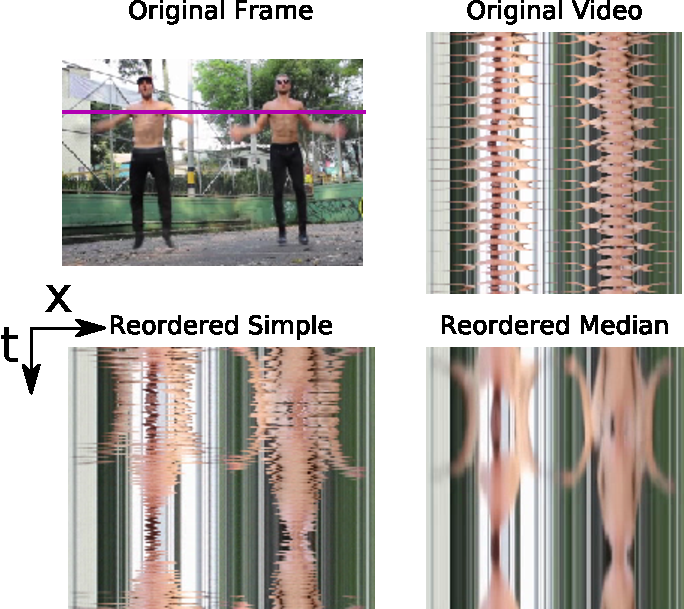
\includegraphics[width=0.8\columnwidth]{XTSlice.pdf}
\caption{An XT slice of a line of pixels (magenta line, upper left) over time for the original video and for reordered videos with and without median consensus.}
\label{fig:XTSlice}
\end{figure}

Figure~\ref{fig:XTSlice} shows the difference between a simple reordering and a median consensus reordering.  Due to natural variation from cycle to cycle, the simple reordering has many temporal discontinuities when interleaving these cycles.  By contrast, the median voting is clean, and it has the added benefit of removing nonperiodic background components.

Advantage of Eulerian is that everything is linear (can use SVD to compress)

Interpolated windows can be projected back to pixel space one by one to save memory (Line~\ref{algline:medianconsensus} of Algorithm~\ref{alg:videoreordering})

\subsection{Sharpening Postprocessing}

The results of the median reordering can be blurry


\section{Experiments}

Robustness experiments, jumping jacks 2 men, two exercise videos from \cite{levy2015live}, beating heart videos from \cite{traliehigh}, \cite{wu2012eulerian}, and \cite{wadhwa2013phase}.


\section{Discussion}

Since we rely on the theory and constructions in \cite{tralie2017quasi}, we are subject to similar constraints in the allowable motion and drift for our method to work well.  We note that Eulerian video magnification also degrades in the presence of too much drift \cite{wu2012eulerian, wadhwa2013phase}.


% References should be produced using the bibtex program from suitable
% BiBTeX files (here: strings, refs, manuals). The IEEEbib.bst bibliography
% style file from IEEE produces unsorted bibliography list.
% -------------------------------------------------------------------------
\bibliographystyle{IEEEbib}
\bibliography{refs}

\end{document}
